% Template:     Informe/Reporte LaTeX
% Documento:    Archivo principal
% Versión:      3.1.3 (17/04/2017)
% Codificación: UTF-8
%
% Autor: Pablo Pizarro R.
%        Facultad de Ciencias Físicas y Matemáticas.
%        Universidad de Chile.
%        pablo.pizarro@ing.uchile.cl, ppizarror.com
%
% Sitio web del proyecto: [http://ppizarror.com/Template-Informe/]
% Licencia: MIT           [https://opensource.org/licenses/MIT]

% CREACIÓN DEL DOCUMENTO, FUENTE E IDIOMA
\documentclass[letterpaper,11pt]{article} % Articulo tamaño carta, fuente 11
\usepackage[utf8]{inputenc}               % Codificación UTF-8
\usepackage[T1]{fontenc}                  % Soporta caracteres acentuados
\usepackage{lmodern}                      % Tipografía moderna
\usepackage[spanish]{babel}               % Idioma del documento en español
\def\templateversion{3.1.3}               % Versión del template
               
% INFORMACIÓN DEL DOCUMENTO
\newcommand{\nombredelinforme}{Square Knight}
\newcommand{\temaatratar}{Juego en 2 Dimensiones: Propuesta Personal.}
\newcommand{\fecharealizacion}{\today}
\newcommand{\fechaentrega}{14 de mayo de 2017}

\newcommand{\autordeldocumento}{Nombre del autor o grupo}
\newcommand{\nombredelcurso}{Modelación y Computación Gráfica para Ingenieros}
\newcommand{\codigodelcurso}{CC-3501}

\newcommand{\nombreuniversidad}{Universidad de Chile}
\newcommand{\nombrefacultad}{Facultad de Ciencias Físicas y Matemáticas}
\newcommand{\departamentouniversidad}{Departamento de la Universidad}
\newcommand{\imagendeldepartamento}{images/departamentos/dcc}
\newcommand{\imagendeldepartamentoescl}{0.2}
\newcommand{\localizacionuniversidad}{Santiago, Chile}

% INTEGRANTES, PROFESORES Y FECHAS
\newcommand{\tablaintegrantes}{
\begin{minipage}{1.0\textwidth}
\begin{flushright}
\begin{tabular}{ll}
	Integrante:
		& \begin{tabular}[t]{@{}l@{}}
			Daniel Soto G.
		\end{tabular} \\
	Profesora:
		& \begin{tabular}[t]{@{}l@{}}
			Nancy Hitschfeld K.
		\end{tabular} \\
	Auxiliares:
		& \begin{tabular}[t]{@{}l@{}}
			Pablo Pizarro R. \\
			Pablo Polanco
		\end{tabular}\\
	Ayudantes:
		& \begin{tabular}[t]{@{}l@{}}
			Joaquín T. Paris \\
			Rodrigo E. Ramos T. \\
			Sergio Leiva
		\end{tabular}\\
	\multicolumn{2}{l}{Fecha de realización: \fecharealizacion} \\
	\multicolumn{2}{l}{Fecha de entrega: \fechaentrega} \\
	\multicolumn{2}{l}{\localizacionuniversidad}
\end{tabular}
\end{flushright}
\end{minipage}}

% CONFIGURACIONES
% Template:     Informe/Reporte LaTeX
% Documento:    Archivo de configuraciones
% Versión:      3.1.3 (17/04/2017)
% Codificación: UTF-8
%
% Autor: Pablo Pizarro R.
%        Facultad de Ciencias Físicas y Matemáticas.
%        Universidad de Chile.
%        pablo.pizarro@ing.uchile.cl, ppizarror.com
%
% Sitio web del proyecto: [http://ppizarror.com/Template-Informe/]
% Licencia: MIT           [https://opensource.org/licenses/MIT]

\newcommand{\defaultimagefolder}{images/}         % Directorio de las imágenes
\newcommand{\defaultnewlinesize}{11pt}            % Tamaño del salto de línea
\newcommand{\defaultinterlind}{1.0}               % Entrelineado por defecto
\newcommand{\tipofuentetitulo}{\huge}             % Tamaño títulos
\newcommand{\tipofuentesubtitulo}{\Large}         % Tamaño subtítulos
\newcommand{\tipofuentesubsubtitulo}{\large}      % Tamaño sub-subtítulos
\newcommand{\tipofuentetituloi}{\huge}            % Tamaño títulos en el índice
\newcommand{\tipofuentesubtituloi}{\Large}        % Tamaño subtítulos en el índice
\newcommand{\tipofuentesubsubtituloi}{\large}     % Tamaño sub-subtit. en el índ.
\newcommand{\etipofuentetitulo}{\bfseries}        % Estilo títulos
\newcommand{\etipofuentesubtitulo}{\bfseries}     % Estilo subtítulos
\newcommand{\etipofuentesubsubtitulo}{\bfseries}  % Estilo sub-subtítulos
\newcommand{\etipofuentetituloi}{\bfseries}       % Estilo títulos en el índice
\newcommand{\etipofuentesubtituloi}{\bfseries}    % Estilo subtítulos en el índice
\newcommand{\etipofuentesubsubtituloi}{\bfseries} % Estilo sub-subti. en el índice
\newcommand{\tiporeferencias}{apa}                % Tipo de referencias
\newcommand{\nomltcontend}{Índice de Contenidos}  % Nombre del índ. de contenidos
\newcommand{\nomlttablas}{Lista de Tablas}        % Nombre de la lista de tablas
\newcommand{\nomltfiguras}{Lista de Figuras}      % Nombre de la lista de figuras
\newcommand{\nomltsrc}{Lista de Códigos Fuente}   % Nombre del código fuente
\newcommand{\nomltwtablas}{Tabla}                 % Nombre de las tablas
\newcommand{\nomltwfigura}{Figura}                % Nombre de las figuras
\newcommand{\nomltwcodfuente}{Código Fuente}      % Nombre del código fuente
\newcommand{\indexdepth}{3}                       % Profundidad del índice
\newcommand{\tablepadding}{1.1}                   % Padding de las tablas
\newcommand{\defaultcaptionmargin}{2.9}           % Márgenes de las leyendas [cm]
\newcommand{\defaultpagemarginleft}{2.5}          % Margen izquierdo página [cm]
\newcommand{\defaultpagemarginright}{2.5}         % Margen derecho página [cm]
\newcommand{\defaultpagemargintop}{3.0}           % Margen superior página [cm]
\newcommand{\defaultpagemarginbottom}{2.7}        % Margen inferior página [cm]
\newcommand{\defaultfirstpagemargintop}{3.8}      % Margen superior portada [cm]
\newcommand{\defaultmarginfloatimages}{-13pt}     % Margen sup. fig. flotante [pt]
\newcommand{\defaultmargintopimages}{0.0cm}       % Margen superior figura [cm]
\newcommand{\defaultmarginbottomimages}{-0.2cm}   % Margen inferior figura [cm]
\newcommand{\defaultcaptionlessmargin}{0.1cm}     % Margen si no hay caption [cm]
\newcommand{\defaultindextitlemargin}{7pt}        % Margen títulos en índice [pt]
\newcommand{\nombrepaginaportada}{Portada}        % Etiqueta página de la portada

% CONFIGURACIONES BOOLEANAS (TRUE, FALSE)
\newcommand{\codigocursoenportada}{false}  % Muestra el código del curso
\newcommand{\showborderonlinks}{false}     % Muestra un recuadro en cada enlace
\newcommand{\showfooter}{true}             % Muestra el footer
\newcommand{\showheadertitle}{true}        % Muestra título de la sección
\newcommand{\showindex}{true}              % Muestra la página del índice
\newcommand{\showindexofcontents}{true}    % Muestra la lista de contenidos
\newcommand{\showindexoffigures}{true}     % Muestra la lista de figuras
\newcommand{\showindexofsourcecode}{false} % Muestra la lista de códigos fuente
\newcommand{\showindexoftables}{true}      % Muestra la lista de tablas
\newcommand{\twocolumnreferences}{false}   % Referencias en dos columnas

% IMPORTACIÓN DE LIBRERÍAS
% Template:     Informe/Reporte LaTeX
% Documento:    Importación de librerías
% Versión:      3.1.3 (17/04/2017)
% Codificación: UTF-8
%
% Autor: Pablo Pizarro R.
%        Facultad de Ciencias Físicas y Matemáticas.
%        Universidad de Chile.
%        pablo.pizarro@ing.uchile.cl, ppizarror.com
%
% Sitio web del proyecto: [http://ppizarror.com/Template-Informe/]
% Licencia: MIT           [https://opensource.org/licenses/MIT]

\usepackage{amsmath}                  % Fórmulas matemáticas
\usepackage{amssymb}                  % Símbolos matemáticos
\usepackage{amsthm}                   % Teoremas matemáticos
\usepackage{array}                    % Añade nuevas características a las tablas
\usepackage{bigstrut}                 % Líneas horizontales en tablas
\usepackage{booktabs}                 % Permite manejar elem. visuales en tablas
\usepackage[makeroom]{cancel}         % Cancelar términos en fórmulas
\usepackage{caption}                  % Leyendas
\usepackage{color}                    % Colores
\usepackage{colortbl}                 % Administración de color en tablas
\usepackage{datetime}                 % Fechas
\usepackage[inline]{enumitem}         % Permite enumerar ítems
\usepackage[bottom, norule]{footmisc} % Estilo pié de página
\usepackage{fancyhdr}                 % Encabezados y pié de páginas
\usepackage{float}                    % Administrador de posiciones de objetos
\usepackage{textcomp, gensymb}        % Simbología común
\usepackage{geometry}                 % Dimensiones y geometría del documento
\usepackage{graphicx}                 % Propiedades extra para los gráficos
\usepackage{ifthen}                   % Permite el manejo de condicionales
\usepackage{mathtools}                % Permite utilizar notaciones matemáticas
\usepackage{multicol}                 % Múltiples columnas
\usepackage{pdfpages}                 % Permite administrar páginas en pdf
\usepackage{lipsum}                   % Permite crear textos dummy
\usepackage{longtable}                % Permite utilizar tablas en varias hojas
\usepackage{listings}                 % Permite añadir código fuente
\usepackage{rotating}                 % Permite rotación de objetos
\usepackage{sectsty}                  % Cambia el estilo de los títulos
\usepackage{selinput}                 % Compatibilidad con acentos
\usepackage{setspace}                 % Cambia el espacio entre líneas
\usepackage{tikz}                     % Permite dibujar
\usepackage{ulem}                     % Permite tachar, subrayar, etc
\usepackage{url}                      % Permite añadir enlaces
\usepackage{wasysym}                  % Contiene caracteres misceláneos
\usepackage{wrapfig}                  % Permite comprimir imágenes
\usepackage{xcolor}                   % Paquete de colores avanzado

% LIBRERÍAS DEPENDIENTES
\usetikzlibrary{babel}                % Asociado a tikz
\usepackage{chngcntr}                 % Agrega números de secciones a las leyendas
\usepackage{epstopdf}                 % Convierte archivos .eps a pdf
\usepackage{multirow}                 % Agrega nuevas opciones a las tablas
\ifthenelse{                          % Permite añadir enlaces y referencias
\equal{\showborderonlinks}{false}}{   % Links sin recuadro rojo
\usepackage[hidelinks]{hyperref}}{
\usepackage{hyperref}}

\usepackage[%
    font={small,sf},
    labelfont=bf,
    format=hang,    
    format=plain,
    margin=0pt,
    width=0.8\textwidth,
]{caption}
\usepackage[list=true]{subcaption}
\usetikzlibrary{automata,positioning}

% IMPORTACIÓN DE FUNCIONES
% Template:     Informe/Reporte LaTeX
% Documento:    Definición de funciones
% Versión:      3.1.3 (17/04/2017)
% Codificación: UTF-8
%
% Autor: Pablo Pizarro R.
%        Facultad de Ciencias Físicas y Matemáticas.
%        Universidad de Chile.
%        pablo.pizarro@ing.uchile.cl, ppizarror.com
%
% Sitio web del proyecto: [http://ppizarror.com/Template-Informe/]
% Licencia: MIT           [https://opensource.org/licenses/MIT]

\newcommand{\throwerror}[2]{
	% Lanza un mensaje de error
	% 	#1	Función del error
	%	#2	Mensaje
	\errmessage{Error: \noexpand#1 #2 (linea \the\inputlineno)}
}

\newcommand{\emptyvarerr}[3]{
	% Lanza un mensaje de error si una variable no ha sido definida
	% 	#1	Función del error
	%	#2	Variable
	%	#3	Mensaje
	\ifx\hfuzz#2\hfuzz
		\throwerror{#1}{#3}
	\fi
}

\newcommand{\quotes}[1]{
	% Insertar cita
	% 	#1	Texto
	''#1''
}

\newcommand{\quotesit}[1]{
	% Insertar cita en itálico
	% 	#1	Texto
	\textit{\quotes{#1}}
}

\newcommand{\newemptypage}{
	% Crea una página vacía
	\newpage\null\thispagestyle{empty}\newpage
	\addtocounter{page}{-1}
}

\newcommand{\setcaptionmargincm}[1]{
	% Cambiar el margen
	% 	#1	Margen en centímetros
	\captionsetup{margin=#1cm}
}

\newcommand{\setpagemargincm}[4]{
	% Cambia márgenes de las páginas [cm]
	% 	#1	Margen izquierdo
	%	#2	Margen superior
	%	#3	Margen derecho
	%	#4	Margen inferior
	\newgeometry{left=#1cm, top=#2cm, right=#3cm, bottom=#4cm}
}

\newcommand{\newp}{
	% Inserta nueva línea	
	\hbadness=10000 \vspace{\defaultnewlinesize} \par
}

\newcommand{\newpar}[1]{
	% Insertar párrafo
	% 	#1	Párrafo
	\hbadness=10000 #1 \newp
}

\newcommand{\newparnl}[1]{
	% Insertar párrafo sin nueva línea al final
	% 	#1	Párrafo
	#1 \par
}

\newcommand{\lpow}[2]{
	% Insertar sub-índice, a_b
	% 	#1	Elemento inferior (a)
	%	#2	Elemento superior (b)
	{#1}_{#2}
}

\newcommand{\pow}[2]{
	% Insertar elevado, a^b
	% 	#1	Elemento inferior (a)
	%	#2	Elemento superior (b)
	{#1}^{#2}
}

\newcommand{\fracpartial}[2]{
	% Fracción de derivadas parciales af/ax
	% 	#1	Función a derivar (f)
	%	#2	Variable a derivar (x)
	\frac{\partial #1}{\partial #2}
}

\newcommand{\fracdpartial}[2]{
	% Fracción de derivadas parciales dobles a^2f/ax^2
	% 	#1	Función a derivar (f)
	%	#2	Variable a derivar (x)
	\frac{{\partial}^{2} #1}{\partial {#2}^{2}}
}

\newcommand{\fracnpartial}[3]{
	% Fracción de derivadas parciales en n, a^nf/ax^n
	% 	#1	Función a derivar (f)
	%	#2	Variable a derivar (x)
	%	#3	Orden (n)
	\frac{{\partial}^{#3} #1}{\partial {#2}^{#3}}
}

\newcommand{\fracderivat}[2]{
	% Fracción de derivadas df/dx
	% 	#1	Función a derivar (f)
	%	#2	Variable a derivar (x)
	\frac{\text{d} #1}{\text{d} #2}
}

\newcommand{\fracdderivat}[2]{
	% Fracción de derivadas dobles d^2/dx^2
	% 	#1	Función a derivar (f)
	%	#2	Variable a derivar (x)
	\frac{{\text{d}}^{2} #1}{\text{d} {#2}^{2}}
}

\newcommand{\fracnderivat}[3]{
	% Fracción de derivadas en n d^nf/dx^n
	% 	#1	Función a derivar (f)
	%	#2	Variable a derivar (x)
	%	#3	Orden de la derivada (n)	
	\frac{{\text{d}}^{#3} #1}{\text{d} {#2}^{#3}}
}

\newcommand{\topequal}[2]{
	% Llave superior de equivalencia
	% 	#1	Elemento a igualar
	%	#2	Igualdad
	\overbrace{#1}^{\mathclap{#2}}
}

\newcommand{\underequal}[2]{
	% Llave inferior de equivalencia
	% 	#1	Elemento a igualar
	%	#2	Igualdad
	\underbrace{#1}_{\mathclap{#2}}
}

\newcommand{\topsequal}[2]{
	% Rectángulo superior de equivalencia
	% 	#1	Elemento a igualar
	%	#2	Igualdad
	\overbracket{#1}^{\mathclap{#2}}
}

\newcommand{\undersequal}[2]{
	% Rectángulo inferior de equivalencia
	% 	#1	Elemento a igualar
	%	#2	Igualdad
	\underbracket{#1}_{\mathclap{#2}}
}

\newcommand{\resizeitem}[2]{
	% Crea un resizebox de tamaño textwidth
	% 	#1	Tamaño del nuevo objeto (En textwidth)
	%	#2	Objeto a redimensionar
	\emptyvarerr{\resizeitem}{#1}{Tamano del nuevo objeto no definido}
	\emptyvarerr{\resizeitem}{#2}{Objeto a redimensionar no definido}
	\resizebox{#1\textwidth}{!}{#2}
}

\newcommand{\newtitleanum}[1]{
	% Insertar un título sin número
	% 	#1	Título
	\emptyvarerr{\newtitleanum}{#1}{Titulo no definido}
	\addcontentsline{toc}{section}{#1}
	\section*{#1}
	\ifthenelse{\equal{\showheadertitle}{true}}{
		\fancyhead[L]{\nouppercase{#1}}}{}
	\stepcounter{section}
}

\newcommand{\newtitleanumheadless}[1]{
	% Insertar un título sin número sin alterar el header
	% 	#1	Título
	\emptyvarerr{\newtitleanumheadless}{#1}{Titulo no definido}
	\addcontentsline{toc}{section}{#1}
	\section*{#1}
	\stepcounter{section}
}

\newcommand{\newsubtitleanum}[1]{
	% Insertar un subtítulo sin número
	% 	#1	Subtítulo
	\emptyvarerr{\newsubtitleanum}{#1}{Subtitulo no definido}
	\addcontentsline{toc}{subsection}{#1}
	\subsection*{#1}
	\stepcounter{subsection}
}

\newcommand{\newsubsubtitleanum}[1]{
	% Insertar un sub-subtítulo sin número
	% 	#1	Sub-subtítulo
	\emptyvarerr{\newsubsubtitleanum}{#1}{Sub-subtitulo no definido}
	\addcontentsline{toc}{subsubsection}{#1}
	\subsubsection*{#1}
	\stepcounter{subsubsection}
}

\newcommand{\newtitleanumnoi}[1]{
	% Insertar un título sin número sin indexar
	% 	#1	Título
	\emptyvarerr{\newtitleanumnoi}{#1}{Titulo no definido}
	\section*{#1}
	\ifthenelse{\equal{\showheadertitle}{true}}{
		\fancyhead[L]{\nouppercase{#1}}}{}
	\stepcounter{section}
}

\newcommand{\newtitleanumnoiheadless}[1]{
	% Insertar un título sin número sin indexar sin cambiar el header
	% 	#1	Título
	\emptyvarerr{\newtitleanumnoiheadless}{#1}{Titulo no definido}
	\section*{#1}
	\ifthenelse{\equal{\showheadertitle}{true}}{
		\fancyhead[L]{\nouppercase{#1}}}{}
	\stepcounter{section}
}

\newcommand{\newsubtitleanumnoi}[1]{
	% Insertar un subtítulo sin número sin indexar
	% 	#1	Subtítulo
	\emptyvarerr{\newsubtitleanumnoi}{#1}{Subtitulo no definido}
	\subsection*{#1}
	\stepcounter{subsection}
}

\newcommand{\newsubsubtitleanumnoi}[1]{
	% Insertar un sub-subtítulo sin número sin indexar
	% 	#1	Sub-subtítulo
	\emptyvarerr{\newsubsubtitleanumnoi}{#1}{Sub-subtitulo no definido}
	\addcontentsline{toc}{subsubsection}{#1}
	\subsubsection*{#1}
	\stepcounter{subsubsection}
}

\newcommand{\insertindextitle}[2]{
	% Insertar un título en un índice
	%	#1	Título
	%	#2	Margen superior en pt. (opcional), 10pt por defecto
	\emptyvarerr{\insertindextitle}{#1}{Titulo no definido}
	\ifx\hfuzz#2\hfuzz
		\addtocontents{toc}{\protect\addvspace{\defaultindextitlemargin}}
	\else
		\addtocontents{toc}{\protect\addvspace{#2 pt}}
	\fi
	\addtocontents{toc}{\noindent\hyperref[swpn]{\textbf{#1}}}
}

\newcommand{\insertequation}[2][]{
	% Insertar una ecuación
	% 	#1	Label (opcional)
	%	#2	Ecuación
	\emptyvarerr{\insertequation}{#2}{Ecuacion no definida}
	\vspace{-0.1cm}
	\begin{equation}
		\text{#1} #2
	\end{equation}
	\vspace{-0.23cm}
	\par
}

\newcommand{\insertequationcaptioned}[3][]{
	% Insertar una ecuación con leyenda
	% 	#1	Label (opcional)
	%	#2	Ecuación
	%	#3	Caption
	\emptyvarerr{\insertequationcaptioned}{#2}{Ecuacion no definida}
	\ifx\hfuzz#3\hfuzz
		\insertequation[#1]{#2}
	\else
		\vspace{0cm}
		\begin{equation}
		\text{#1} #2
		\end{equation}
		\begin{center}
			\vspace{-0.15cm}
			\textit{#3} \par
			\vspace{0.05cm}
		\end{center}	
	\fi
}

\newcommand{\insertequationgathered}[2][]{
	% Insertar una ecuación con el ambiente gather
	% 	#1	Label (opcional)
	%	#2	Ecuación
	\emptyvarerr{\insertequationgathered}{#2}{Ecuacion no definida}
	\vspace{-0.4cm}
	\begin{gather}
		\text{#1} #2
	\end{gather}
	\par
	\vspace{-0.10cm}
}

\newcommand{\insertequationgatheredcaptioned}[3][]{
	% Insertar una ecuación (gather) con leyenda
	% 	#1	Label (opcional)
	%	#2	Ecuación
	%	#3	Caption
	\emptyvarerr{\insertequationgatheredcaptioned}{#2}{Ecuacion no definida}
	\ifx\hfuzz#3\hfuzz
		\insertequationgathered[#1]{#2}
	\else
		\vspace{0cm}
		\begin{gather}
			\text{#1} #2
		\end{gather}
		\begin{center}
			\vspace{-0.15cm}
			\textit{#3} \par
		\end{center}
	\fi
}

\newcommand{\insertequationalign}[2][]{
	% Insertar una ecuación con el ambiente align
	% 	#1	Label (opcional)
	%	#2	Ecuación
	\emptyvarerr{\insertequationalign}{#2}{Ecuacion no definida}
	\vspace{-0.4cm}
	\begin{align}
		\text{#1} #2
	\end{align}
	\par
	\vspace{-0.10cm}
}

\newcommand{\insertequationaligncaptioned}[3][]{
	% Insertar una ecuación (align) con leyenda
	% 	#1	Label (opcional)
	%	#2	Ecuación
	%	#3	Caption
	\emptyvarerr{\insertequationaligncaptioned}{#2}{Ecuacion no definida}
	\ifx\hfuzz#3\hfuzz
		\insertequationalign[#1]{#2}
	\else
		\vspace{0cm}
		\begin{align}
			\text{#1} #2
		\end{align}
		\begin{center}
			\vspace{-0.15cm}
			\textit{#3} \par
		\end{center}
	\fi
}

\newcommand{\insertimage}[4][]{
	% Insertar una imagen
	% 	#1	Label (opcional)
	%	#2	Dirección de la imagen
	%	#3	Parámetros de la imagen
	%	#4	Caption de la imagen
	\emptyvarerr{\insertimage}{#2}{Direccion de la imagen no definida}
	\emptyvarerr{\insertimage}{#3}{Parametros de la imagen no definidos}
	\vspace{\defaultmargintopimages}
	\begin{figure}[H]
		\centering
		\includegraphics[#3]{\defaultimagefolder#2}
		\ifx\hfuzz#4\hfuzz
			\vspace{\defaultcaptionlessmargin}
		\else
			\caption{#4 #1}
		\fi
	\end{figure}
	\vspace{\defaultmarginbottomimages}
}

\newcommand{\insertimageboxed}[4][]{
	% Insertar una imagen con recuadro
	% 	#1	Label (opcional)
	%	#2	Dirección de la imagen
	%	#3	Parámetros de la imagen
	%	#4	Caption de la imagen
	\emptyvarerr{\insertimageboxed}{#2}{Direccion de la imagen no definida}
	\emptyvarerr{\insertimageboxed}{#3}{Parametros de la imagen no definidos}
	\vspace{\defaultmargintopimages}
	\begin{figure}[H]
		\centering
		\fbox{\includegraphics[#3]{\defaultimagefolder#2}}
		\ifx\hfuzz#4\hfuzz
			\vspace{\defaultcaptionlessmargin}
		\else
			\caption{#4 #1}
		\fi
	\end{figure}
	\vspace{\defaultmarginbottomimages}
}

\newcommand{\insertimagefixed}[5][]{
	% Insertar una imagen de ancho fijo a la página
	% 	#1	Label (opcional)
	%	#2	Dirección de la imagen
	%	#3	Parámetros de la imagen
	%	#4	Tamaño de la imagen en textwidth
	%	#5	Caption de la imagen
	\emptyvarerr{\insertimagefixed}{#2}{Direccion de la imagen no definida}
	\emptyvarerr{\insertimagefixed}{#3}{Parametros de la imagen no definidos}
	\emptyvarerr{\insertimagefixed}{#4}{Tamano de la imagen (textwidth) no definida}
	\vspace{\defaultmargintopimages}
	\begin{figure}[H]
		\centering
		\resizebox{#3\textwidth}{!}{
			\includegraphics[#4]{\defaultimagefolder#2}
		}
		\ifx\hfuzz#5\hfuzz
			\vspace{\defaultcaptionlessmargin}
		\else
			\caption{#5 #1}
		\fi
	\end{figure}
	\vspace{\defaultmarginbottomimages}
}

\newcommand{\insertimageboxedfixed}[5][]{
	% Insertar una imagen recuadrada de ancho fijo
	% 	#1	Label (opcional)
	%	#2	Dirección de la imagen
	%	#3	Parámetros de la imagen
	%	#4	Tamaño de la imagen en textwidth
	%	#5	Caption de la imagen
	\emptyvarerr{\insertimageboxedfixed}{#2}{Direccion de la imagen no definida}
	\emptyvarerr{\insertimageboxedfixed}{#3}{Parametros de la imagen no definidos}
	\emptyvarerr{\insertimageboxedfixed}{#4}{Tamano de la imagen no definida}
	\vspace{\defaultmargintopimages}
	\begin{figure}[H]
		\centering
		\resizebox{#3\textwidth}{!}{
			\fbox{\includegraphics[#4]{\defaultimagefolder#2}}
		}
		\ifx\hfuzz#5\hfuzz
			\vspace{\defaultcaptionlessmargin}
		\else
			\caption{#5 #1}
		\fi
	\end{figure}
	\vspace{\defaultmarginbottomimages}
}

\newcommand{\insertdoubleimage}[8][]{
	% Insertar una imagen doble
	% 	#1	Label (opcional)
	%	#2	Dirección de la imagen 1
	%	#3	Parámetros de la imagen 1
	%	#4	Caption de la imagen 1
	%	#5	Dirección de la imagen 2
	%	#6	Parámetros de la imagen 2
	%	#7	Caption de la imagen 2
	%	#8	Caption de la imagen doble
	\emptyvarerr{\insertdoubleimage}{#2}{Direccion de la imagen 1 no definida}
	\emptyvarerr{\insertdoubleimage}{#3}{Parametros de la imagen 1 no definidos}
	\emptyvarerr{\insertdoubleimage}{#5}{Direccion de la imagen 2 no definida}
	\emptyvarerr{\insertdoubleimage}{#6}{Parametros de la imagen 2 no definidos}
	\vspace{\defaultmargintopimages}
	\captionsetup{margin=0.45cm}
	\begin{figure}[H] \centering
		\subfloat[#4]{
			\includegraphics[#3]{\defaultimagefolder#2}}
		\hspace{0.2cm}
		\subfloat[#7]{
			\includegraphics[#6]{\defaultimagefolder#5}}
		\setcaptionmargincm{\defaultcaptionmargin}
		\ifx\hfuzz#8\hfuzz
			\vspace{\defaultcaptionlessmargin}
		\else
			\caption{#8 #1}
		\fi
	\end{figure}
	\setcaptionmargincm{\defaultcaptionmargin}
	\vspace{\defaultmarginbottomimages}
}

\newcommand{\insertdoubleeqimage}[7][]{
	% Insertar una imagen doble, igual propiedades
	% 	#1	Label (opcional)
	%	#2	Dirección de la imagen 1
	%	#3	Caption de la imagen 1
	%	#4	Dirección de la imagen 2
	%	#5	Caption de la imagen 2
	%	#6	Propiedades de las imágenes
	%	#7 	Caption de la imagen doble
	\insertdoubleimage[#1]{#2}{#6}{#3}{#4}{#6}{#5}{#7}
}

\newcommand{\inserttripleimage}[8][]{
	% Insertar una imagen triple
	% 	#1	Label (opcional)
	%	#2	Dirección de la imagen 1
	%	#3	Parámetros de la imagen 1
	%	#4	Dirección de la imagen 2
	%	#5	Parámetros de la imagen 2
	%	#6	Dirección de la imagen 3
	%	#7	Parámetros de la imagen 3
	%	#8	Caption de la imagen triple
	\emptyvarerr{\inserttripleimage}{#2}{Direccion de la imagen 1 no definida}
	\emptyvarerr{\inserttripleimage}{#3}{Parametros de la imagen 1 no definidos}
	\emptyvarerr{\inserttripleimage}{#4}{Direccion de la imagen 2 no definida}
	\emptyvarerr{\inserttripleimage}{#5}{Parametros de la imagen 2 no definidos}
	\emptyvarerr{\inserttripleimage}{#6}{Direccion de la imagen 3 no definida}
	\emptyvarerr{\inserttripleimage}{#7}{Parametros de la imagen 3 no definidos}
	\vspace{\defaultmargintopimages}
	\captionsetup{margin=0.45cm}
	\begin{figure}[H] \centering
		\subfloat[]{
			\includegraphics[#3]{\defaultimagefolder#2}}
		\hspace{0.1cm}
		\subfloat[]{
			\includegraphics[#5]{\defaultimagefolder#4}}
		\hspace{0.1cm}
		\subfloat[]{
			\includegraphics[#7]{\defaultimagefolder#6}}
		\setcaptionmargincm{\defaultcaptionmargin}
		\ifx\hfuzz#8\hfuzz
			\vspace{\defaultcaptionlessmargin}
		\else
			\caption{#8 #1}
		\fi
	\end{figure}
	\setcaptionmargincm{\defaultcaptionmargin}
	\vspace{\defaultmarginbottomimages}
}

\newcommand{\inserttripleeqimage}[6][]{
	% Insertar una imagen triple, igual propiedades
	% 	#1	Label (opcional)
	%	#2	Dirección de la imagen 1
	%	#3	Dirección de la imagen 2
	%	#4	Dirección de la imagen 3
	%	#5	Propiedades de las imágenes
	%	#6	Caption de la imagen triple
	\inserttripleimage[#1]{#2}{#5}{#3}{#5}{#4}{#5}{#6}
}

\newcommand{\insertquadimage}[7][]{
	% Insertar una imagen cuádruple, igual propiedades
	% 	#1	Label (opcional)
	%	#2	Dirección de la imagen 1
	%	#3	Dirección de la imagen 2
	%	#4	Dirección de la imagen 3
	%	#5	Dirección de la imagen 4
	%	#6	Propiedades de las imágenes
	%	#7	Caption de la imagen cuádruple
	\emptyvarerr{\insertquadimage}{#2}{Direccion de la imagen 1 no definida}
	\emptyvarerr{\insertquadimage}{#3}{Direccion de la imagen 2 no definida}
	\emptyvarerr{\insertquadimage}{#4}{Direccion de la imagen 3 no definida}
	\emptyvarerr{\insertquadimage}{#5}{Direccion de la imagen 4 no definida}
	\emptyvarerr{\insertquadimage}{#6}{Propiedades de las imagenes no definidos}
	\vspace{\defaultmargintopimages}
	\captionsetup{margin=0.45cm}
	\begin{figure}[H] \centering
		\subfloat[]{
			\includegraphics[#6]{\defaultimagefolder#2}}
		\hspace{0.1cm}
		\subfloat[]{
			\includegraphics[#6]{\defaultimagefolder#3}}
		\hspace{0.1cm}
		\subfloat[]{
			\includegraphics[#6]{\defaultimagefolder#4}}
		\hspace{0.1cm}
		\subfloat[]{
			\includegraphics[#6]{\defaultimagefolder#5}}
		\setcaptionmargincm{\defaultcaptionmargin}
		\ifx\hfuzz#7\hfuzz
			\vspace{\defaultcaptionlessmargin}
		\else
			\caption{#7 #1}
		\fi
	\end{figure}
	\setcaptionmargincm{\defaultcaptionmargin}
	\vspace{\defaultmarginbottomimages}
}

\newcommand{\insertpentaimage}[8][]{
	% Insertar una imagen quíntuple, igual propiedades
	% 	#1	Label (opcional)
	%	#2	Dirección de la imagen 1
	%	#3	Dirección de la imagen 2
	%	#4	Dirección de la imagen 3
	%	#5	Dirección de la imagen 4
	%	#6	Dirección de la imagen 5
	%	#7	Propiedades de las imágenes
	%	#8	Caption de la imagen quíntuple
	\emptyvarerr{\insertpentaimage}{#2}{Direccion de la imagen 1 no definida}
	\emptyvarerr{\insertpentaimage}{#3}{Direccion de la imagen 2 no definida}
	\emptyvarerr{\insertpentaimage}{#4}{Direccion de la imagen 3 no definida}
	\emptyvarerr{\insertpentaimage}{#5}{Direccion de la imagen 4 no definida}
	\emptyvarerr{\insertpentaimage}{#6}{Direccion de la imagen 5 no definida}
	\emptyvarerr{\insertpentaimage}{#7}{Propiedades de las imagenes no definidas}
	\vspace{\defaultmargintopimages}
	\captionsetup{margin=0.45cm}
	\begin{figure}[H] \centering
		\subfloat[]{
			\includegraphics[#7]{\defaultimagefolder#2}}
		\hspace{0.1cm}
		\subfloat[]{
			\includegraphics[#7]{\defaultimagefolder#3}}
		\hspace{0.1cm}
		\subfloat[]{
			\includegraphics[#7]{\defaultimagefolder#4}}
		\hspace{0.1cm}
		\subfloat[]{
			\includegraphics[#7]{\defaultimagefolder#5}}
		\hspace{0.1cm}
		\subfloat[]{
			\includegraphics[#7]{\defaultimagefolder#6}}
		\setcaptionmargincm{\defaultcaptionmargin}
		\ifx\hfuzz#8\hfuzz
			\vspace{\defaultcaptionlessmargin}
		\else
			\caption{#8 #1}
		\fi
	\end{figure}
	\setcaptionmargincm{\defaultcaptionmargin}
	\vspace{\defaultmarginbottomimages}
}

\newcommand{\inserthexaimage}[9][]{
	% Insertar una imagen con 6 imágenes, igual propiedades
	% 	#1	Label (opcional)
	%	#2	Dirección de la imagen 1
	%	#3	Dirección de la imagen 2
	%	#4	Dirección de la imagen 3
	%	#5	Dirección de la imagen 4
	%	#6	Dirección de la imagen 5
	%	#7	Dirección de la imagen 6
	%	#8	Propiedades de las imágenes
	%	#9	Caption de la imagen global
	\emptyvarerr{\inserthexaimage}{#2}{Direccion de la imagen 1 no definida}
	\emptyvarerr{\inserthexaimage}{#3}{Direccion de la imagen 2 no definida}
	\emptyvarerr{\inserthexaimage}{#4}{Direccion de la imagen 3 no definida}
	\emptyvarerr{\inserthexaimage}{#5}{Direccion de la imagen 4 no definida}
	\emptyvarerr{\inserthexaimage}{#6}{Direccion de la imagen 5 no definida}
	\emptyvarerr{\inserthexaimage}{#7}{Direccion de la imagen 6 no definida}
	\emptyvarerr{\inserthexaimage}{#8}{Propiedades de las imagenes no definidas}
	\vspace{\defaultmargintopimages}
	\captionsetup{margin=0.45cm}
	\begin{figure}[H] \centering
		\subfloat[]{
			\includegraphics[#8]{\defaultimagefolder#2}}
		\hspace{0.1cm}
		\subfloat[]{
			\includegraphics[#8]{\defaultimagefolder#3}}
		\hspace{0.1cm}
		\subfloat[]{
			\includegraphics[#8]{\defaultimagefolder#4}}
		\hspace{0.1cm}
		\subfloat[]{
			\includegraphics[#8]{\defaultimagefolder#5}}
		\hspace{0.1cm}
		\subfloat[]{
			\includegraphics[#8]{\defaultimagefolder#6}}
		\hspace{0.1cm}
		\subfloat[]{
			\includegraphics[#8]{\defaultimagefolder#7}}
		\setcaptionmargincm{\defaultcaptionmargin}
		\ifx\hfuzz#9\hfuzz
			\vspace{\defaultcaptionlessmargin}
		\else
			\caption{#9 #1}
		\fi
	\end{figure}
	\setcaptionmargincm{\defaultcaptionmargin}
	\vspace{\defaultmarginbottomimages}
}

\newcommand{\insertimageleft}[5][]{
	% Insertar una imagen a la izquierda
	% 	#1	Label (opcional)
	%	#2	Dirección de la imagen
	%	#3	Ancho de la imagen (en textwidth)
	%	#4	Altura en líneas de la imagen
	%	#5	Caption de la imagen
	\emptyvarerr{\insertimageleft}{#2}{Direccion de la imagen no definida}
	\emptyvarerr{\insertimageleft}{#3}{Ancho de la imagen no defindo}
	\emptyvarerr{\insertimageleft}{#4}{Altura en lineas de la imagen no definida}
	\begin{wrapfigure}[#4]{l}{#3\textwidth}
		\setcaptionmargincm{0}
		\vspace{\defaultmarginfloatimages}
		\centering
		\includegraphics[width=\linewidth]{\defaultimagefolder#2}
		\ifx\hfuzz#5\hfuzz
			\vspace{\defaultcaptionlessmargin}
		\else
			\caption{#5 #1}
		\fi
		\setcaptionmargincm{\defaultcaptionmargin}
	\end{wrapfigure}
}

\newcommand{\insertimageright}[5][]{
	% Insertar una imagen a la derecha
	% 	#1	Label (opcional)
	%	#2	Dirección de la imagen
	%	#3	Ancho de la imagen (en textwidth)
	%	#4	Altura en líneas de la imagen
	%	#5	Caption de la imagen
	\emptyvarerr{\insertimageright}{#2}{Direccion de la imagen no definida}
	\emptyvarerr{\insertimageright}{#3}{Ancho de la imagen no defindo}
	\emptyvarerr{\insertimageright}{#4}{Altura en lineas de la imagen no definida}
	\begin{wrapfigure}[#4]{r}{#3\textwidth}
		\setcaptionmargincm{0}
		\vspace{\defaultmarginfloatimages}
		\centering
		\includegraphics[width=\linewidth]{\defaultimagefolder#2}
		\ifx\hfuzz#5\hfuzz
			\vspace{\defaultcaptionlessmargin}
		\else
			\caption{#5 #1}
		\fi
		\setcaptionmargincm{\defaultcaptionmargin}
	\end{wrapfigure}
}

% IMPORTACIÓN DE AMBIENTES Y ESTILOS
% Template:     Informe/Reporte LaTeX
% Documento:    Definición de estilos
% Versión:      3.1.3 (17/04/2017)
% Codificación: UTF-8
%
% Autor: Pablo Pizarro R.
%        Facultad de Ciencias Físicas y Matemáticas.
%        Universidad de Chile.
%        pablo.pizarro@ing.uchile.cl, ppizarror.com
%
% Sitio web del proyecto: [http://ppizarror.com/Template-Informe/]
% Licencia: MIT           [https://opensource.org/licenses/MIT]

% Definición de colores
\definecolor{dkgreen}{rgb}{0,0.6,0}
\definecolor{gray}{rgb}{0.5,0.5,0.5}
\definecolor{mauve}{rgb}{0.58,0,0.82}
\definecolor{mygreen}{rgb}{0,0.6,0}
\definecolor{mygray}{rgb}{0.5,0.5,0.5}
\definecolor{mymauve}{rgb}{0.58,0,0.82}
\definecolor{codegreen}{rgb}{0,0.6,0}
\definecolor{codegray}{rgb}{0.5,0.5,0.5}
\definecolor{codepurple}{rgb}{0.58,0,0.82}
\definecolor{backcolour}{rgb}{0.95,0.95,0.92}

% Columna centrada en tablas
\newcolumntype{P}[1]{
	>{\centering\arraybackslash}p{#1}
}

% Definición de acentos
\SelectInputMappings{
	aacute={á},
	Ntilde={Ñ},
	Euro={€}
}

% Estilo de lenguaje C
\lstdefinestyle{C}{
	language=C,
	numbers=left,
	stepnumber=1,
	numbersep=5pt,
	backgroundcolor=\color{white},
	showspaces=false,
	showstringspaces=false,
	showtabs=false,
	tabsize=2,
	captionpos=b,
	breaklines=true,
	breakatwhitespace=true,
	title=\lstname
}

% Estilo de lenguaje Java
\lstdefinestyle{Java}{
	language=Java,
	aboveskip=3mm,
	belowskip=3mm,
	showstringspaces=false,
	columns=flexible,
	basicstyle={\small\ttfamily},
	numbers=left,
	numberstyle=\tiny\color{gray},
	keywordstyle=\color{blue},
	commentstyle=\color{dkgreen},
	stringstyle=\color{mauve},
	breaklines=true,
	breakatwhitespace=true,
	tabsize=3,
	backgroundcolor=\color{backcolour}
}

% Estilo de lenguaje Matlab
\lstdefinestyle{Matlab}{
	language=Matlab,
	breaklines=true,
	morekeywords={matlab2tikz},
	keywordstyle=\color{blue},
	morekeywords=[2]{1}, keywordstyle=[2]{\color{black}},
	backgroundcolor=\color{backcolour},
	identifierstyle=\color{black},
	stringstyle=\color{mylilas},
	commentstyle=\color{mygreen},
	showstringspaces=false,
	numbers=left,
	showstringspaces=false,
	numberstyle=\tiny\color{gray},
	numbersep=9pt,
	basicstyle={\small\ttfamily},
	tabsize=3,
	breaklines=true,
	aboveskip=3mm,
	belowskip=3mm,
	emph=[1]{for,end,break},emphstyle=[1]\color{red}
}

% Estilo de lenguaje Python
\lstdefinestyle{Python}{
	language=Python,
	backgroundcolor=\color{backcolour},
	commentstyle=\color{codegreen},
	keywordstyle=\color{magenta},
	numberstyle=\tiny\color{codegray},
	stringstyle=\color{codepurple},
	basicstyle=\footnotesize,
	breakatwhitespace=false,
	breaklines=true,
	captionpos=b,
	keepspaces=true,
	numbers=left,
	numbersep=5pt,
	showspaces=false,
	showstringspaces=false,
	showtabs=false,
	tabsize=3,
	basicstyle={\small\ttfamily}
}

% Se definen acentos de carácteres especiales
\lstset{literate=
	{á}{{\'a}}1 {é}{{\'e}}1 {í}{{\'i}}1 {ó}{{\'o}}1 {ú}{{\'u}}1
	{Á}{{\'A}}1 {É}{{\'E}}1 {Í}{{\'I}}1 {Ó}{{\'O}}1 {Ú}{{\'U}}1
	{à}{{\`a}}1 {è}{{\`e}}1 {ì}{{\`i}}1 {ò}{{\`o}}1 {ù}{{\`u}}1
	{À}{{\`A}}1 {È}{{\'E}}1 {Ì}{{\`I}}1 {Ò}{{\`O}}1 {Ù}{{\`U}}1
	{ä}{{\"a}}1 {ë}{{\"e}}1 {ï}{{\"i}}1 {ö}{{\"o}}1 {ü}{{\"u}}1
	{Ä}{{\"A}}1 {Ë}{{\"E}}1 {Ï}{{\"I}}1 {Ö}{{\"O}}1 {Ü}{{\"U}}1
	{â}{{\^a}}1 {ê}{{\^e}}1 {î}{{\^i}}1 {ô}{{\^o}}1 {û}{{\^u}}1
	{Â}{{\^A}}1 {Ê}{{\^E}}1 {Î}{{\^I}}1 {Ô}{{\^O}}1 {Û}{{\^U}}1
	{œ}{{\oe}}1 {Œ}{{\OE}}1 {æ}{{\ae}}1 {Æ}{{\AE}}1 {ß}{{\ss}}1
	{ű}{{\H{u}}}1 {Ű}{{\H{U}}}1 {ő}{{\H{o}}}1 {Ő}{{\H{O}}}1
	{ç}{{\c c}}1 {Ç}{{\c C}}1 {ø}{{\o}}1 {å}{{\r a}}1 {Å}{{\r A}}1
	{€}{{\EUR}}1 {£}{{\pounds}}1
}

% CONFIGURACIÓN INICIAL DEL DOCUMENTO
% Template:     Informe/Reporte LaTeX
% Documento:    Configuración inicial del template
% Versión:      3.1.3 (17/04/2017)
% Codificación: UTF-8
%
% Autor: Pablo Pizarro R.
%        Facultad de Ciencias Físicas y Matemáticas.
%        Universidad de Chile.
%        pablo.pizarro@ing.uchile.cl, ppizarror.com
%
% Sitio web del proyecto: [http://ppizarror.com/Template-Informe/]
% Licencia: MIT           [https://opensource.org/licenses/MIT]

\decimalpoint                        % Se define el punto decimal
\counterwithin{equation}{section}    % Añade número de sección a las ecuaciones
\counterwithin{figure}{section}      % Añade número de sección a las figuras
\counterwithin{table}{section}       % Añade número de sección a las tablas
\bibliographystyle{\tiporeferencias} % Estilo APA para las referencias
\setlength{\headheight}{64pt}        % Tamaño de la cabecera sin fancyhdr
\setcounter{tocdepth}{\indexdepth}   % Se ajusta la profundidad del índice
\setcounter{MaxMatrixCols}{20}       % Número máximo de columnas en matrices
\hypersetup{
	pdfauthor={\autordeldocumento},
	pdftitle={\nombredelinforme},
	pdfsubject={\temaatratar},
	pdfkeywords={\nombreuniversidad, \nombredelcurso,
	\codigodelcurso, \localizacionuniversidad},
	pdfcreator={pdfLaTeX, ppizarror},
	pdfproducer={Template LaTeX informe v\templateversion}}
\renewcommand{\baselinestretch}{\defaultinterlind} % Ajuste del entrelineado
\setcaptionmargincm{\defaultcaptionmargin}         % Margen por defecto
\makeatletter
\ifthenelse{\equal{\twocolumnreferences}{true}}{
	% Bibliografía en 2 columnas
	\renewenvironment{thebibliography}[1]
	{\begin{multicols}{2}[\section*{\refname}]
		\@mkboth{\MakeUppercase\refname}{\MakeUppercase\refname}
		\list{\@biblabel{\@arabic\c@enumiv}}
		{\settowidth\labelwidth{\@biblabel{#1}}
			\leftmargin\labelwidth
			\advance\leftmargin\labelsep
			\@openbib@code
			\usecounter{enumiv}
			\let\p@enumiv\@empty
			\renewcommand\theenumiv{\@arabic\c@enumiv}}
		\sloppy
		\clubpenalty 4000
		\@clubpenalty \clubpenalty
		\widowpenalty 4000
		\sfcode`\.\@m}
		{\def\@noitemerr
		{\@latex@warning{Ambiente `thebibliography' no definido}}
		\endlist\end{multicols}}}{}
\makeatother

% PORTADA
\begin{document}
% Template:     Informe/Reporte LaTeX
% Documento:    Portada
% Versión:      3.1.3 (17/04/2017)
% Codificación: UTF-8
%
% Autor: Pablo Pizarro R.
%        Facultad de Ciencias Físicas y Matemáticas.
%        Universidad de Chile.
%        pablo.pizarro@ing.uchile.cl, ppizarror.com
%
% Sitio web del proyecto: [http://ppizarror.com/Template-Informe/]
% Licencia: MIT           [https://opensource.org/licenses/MIT]

\newpage
\renewcommand{\thepage}{\nombrepaginaportada}
\setpagemargincm{\defaultpagemarginleft}{\defaultfirstpagemargintop}
{\defaultpagemarginright}{\defaultpagemarginbottom}
\pagestyle{fancy}
\fancyhf{}
\fancyhead[L]{
\nombreuniversidad \\ \nombrefacultad \\ \departamentouniversidad}
\fancyhead[R]{
\includegraphics[scale=\imagendeldepartamentoescl]{\imagendeldepartamento}}

% Estilo que muestra el código en la portada
\ifthenelse{\equal{\codigocursoenportada}{true}}{
	\vspace*{3cm}
	\begin{center}
		\huge {\nombredelcurso} \\
		\vspace{0.3cm}
		\large {Código del curso: \codigodelcurso} \\
		\vspace{1.5cm}
		\Huge {\nombredelinforme} \\
		\vspace{0.3cm}
		\large {\temaatratar}
	\end{center}

% Estilo normal
}{
	\vspace*{5cm}
	\begin{center}
		\huge {\nombredelcurso} \\
		\vspace{1cm}
		\Huge {\nombredelinforme} \\
		\vspace{0.3cm}
		\large {\temaatratar}
	\end{center}
}

\vfill
\tablaintegrantes

% CONFIGURACIÓN DE PÁGINA Y ENCABEZADOS
% Template:     Informe/Reporte LaTeX
% Documento:    Configuración de página
% Versión:      3.1.3 (17/04/2017)
% Codificación: UTF-8
%
% Autor: Pablo Pizarro R.
%        Facultad de Ciencias Físicas y Matemáticas.
%        Universidad de Chile.
%        pablo.pizarro@ing.uchile.cl, ppizarror.com
%
% Sitio web del proyecto: [http://ppizarror.com/Template-Informe/]
% Licencia: MIT           [https://opensource.org/licenses/MIT]

% Se crea la numeración y los márgenes
\newpage \pagenumbering{Roman}
\setcounter{page}{1}
\setcounter{footnote}{1}
\setpagemargincm{\defaultpagemarginleft}{\defaultpagemargintop}
{\defaultpagemarginright}{\defaultpagemarginbottom}
\def\arraystretch{\tablepadding} % Se ajusta el padding de las tablas

% Definición de nombres a objetos
\renewcommand{\sectionmark}[1]{\markboth{#1}{}} % Se modifica el estilo del header
\renewcommand{\listfigurename}{\nomltfiguras} % Nombre del índice de figuras
\renewcommand{\listtablename}{\nomlttablas} % Nombre del índice de tablas
\renewcommand{\contentsname}{\nomltcontend} % Nombre del índice
\renewcommand{\lstlistlistingname}{\nomltsrc} % Nombre índice código fuente
\renewcommand{\tablename}{\nomltwtablas} % Nombre de la leyenda de las tablas
\renewcommand{\figurename}{\nomltwfigura} % Nombre de la leyenda de las figuras
\renewcommand{\lstlistingname}{\nomltsrc} % Nombre leyenda del código fuente

% Se crean los estílos de página
\pagestyle{fancy} \fancyhf{} % Se crean los headers y footers
\ifthenelse{\equal{\showheadertitle}{true}}{ % Header izq, nombre sección
	\fancyhead[L]{\nouppercase{\rightmark}}
}{}
\fancyhead[R]{\small \rm \nouppercase{\thepage}} % Header der, número página
\ifthenelse{\equal{\showfooter}{true}}{
	\fancyfoot[L]{
		\small \rm \textit{\nombredelinforme} % Footer izq, título del informe
	}
	\fancyfoot[R]{
		\small \rm \textit{\codigodelcurso \ \nombredelcurso} % Footer der, curso
	}
	\renewcommand{\footrulewidth}{0.5pt} % Ancho de la barra del footer
}{}
\renewcommand{\headrulewidth}{0.5pt} % Ancho de la barra del header
\sectionfont{
	\tipofuentetitulo \etipofuentetitulo \selectfont % Tipo de título para abstract
}

% RESUMEN O ABSTRACT
% Template:     Informe/Reporte LaTeX
% Documento:    Abstract o Resumen
% Versión:      3.1.3 (17/04/2017)
% Codificación: UTF-8
%
% Autor: Pablo Pizarro R.
%        Facultad de Ciencias Físicas y Matemáticas.
%        Universidad de Chile.
%        pablo.pizarro@ing.uchile.cl, ppizarror.com
%
% Sitio web del proyecto: [http://ppizarror.com/Template-Informe/]
% Licencia: MIT           [https://opensource.org/licenses/MIT]

\newtitleanumheadless{Resumen}

Este informe trata sobre el desarrollo de un juego arcade de accion y plataformas. Se usaron funciones de colisión incluidas en pygame y se implementaron distintas funciones para colisionar con el nivel. Se generan además power-ups al azar y enemigos con una IA básica. Los objetivo principales se cumplieron satisfactoriamente, y fueron implementados con una serie de clases que permiten la extensión a otras estructuras de niveles y nuevos tipos de enemigos o power-ups. % Se incluye un ejemplo de resumen, se puede borrar

% CONFIGURACIONES FINALES - INICIO DE LAS SECCIONES
% Template:     Informe/Reporte LaTeX
% Documento:    Archivo principal
% Versión:      3.1.3 (17/04/2017)
% Codificación: UTF-8
%
% Autor: Pablo Pizarro R.
%        Facultad de Ciencias Físicas y Matemáticas.
%        Universidad de Chile.
%        pablo.pizarro@ing.uchile.cl, ppizarror.com
%
% Sitio web del proyecto: [http://ppizarror.com/Template-Informe/]
% Licencia: MIT           [https://opensource.org/licenses/MIT]

\newpage
\ifthenelse{
	\equal{\showheadertitle}{true}}{\fancyhead[L]{\nouppercase{\leftmark}}}{}
\sectionfont{\tipofuentetitulo \etipofuentetitulo \selectfont}
\subsectionfont{\tipofuentesubtitulo \etipofuentesubtitulo \selectfont}
\subsubsectionfont{\tipofuentesubsubtitulo \etipofuentesubsubtitulo \selectfont}
\renewcommand{\thepage}{\arabic{page}}
\setcounter{page}{1}
\setcounter{section}{0}
\setcounter{footnote}{0}

% ======================== INICIO DEL DOCUMENTO ========================
\section{Introducción}
	El problema planteado es generar un juego de acción y plataformas en dos dimensiones. El juego debe permitir al usuario controlar a un personaje con total libertad para moverse dentro de la pantalla. Este personaje debe ser capaz de moverse hacia los lados, saltar y atacar. En la escena deben aparecer enemigos al azar, los cuales tienen que ser capaces de seguir al jugador, sin importar su posición en el nivel. Un sistema para encontrar colisiones es necesario. Al hacer y recibir daño se tienen que reproducir sonidos, al igual que al saltar. Deben haber representaciones gráficas de los puntos de vida del jugador y su puntaje, visibles durante el loop principal del juego.

\section{Solución}
	La modelación del juego fue realizada a través de las siguientes clases:
	\renewcommand{\theenumii}{\roman{enumii}}
	\begin{enumerate}
		\item \verb!Platform!:
		Esta clase modela una plataforma rectangular en el nivel. Tiene métodos para encontrar su posición relativa con respecto a cierta \verb!Entidad!.
		\item \verb!Level!:
		Esta clase modela un nivel con un conjunto de \verb!Plataformas!, dándoles un mismo color a todas. Incluye un método \verb!draw()! para dibujar en la vista todas las plataformas.
		\item \verb!Entity!:
		Ambos el jugador y los enemigos heredan de esta clase. Contiene métodos para moverse hacia la izquierda y la derecha y saltar. También actualiza la coordenada vertical con respecto al conjunto de platformas del nivel, con tal de evitar que la entidad entre a una plataforma. Para las coordenadas horizontales, esto se maneja en las métodos de movimiento lateral. Además se incluyen métodos auxiliares booleanos y de estado, para simplificar los condicionales en los métodos de esta clase. Finalmente, incluye métodos para dibujar a la entidad en la vista.
		\begin{enumerate}
			\item \verb!Player!:
			Esta clase contiene métodos para atacar, booleanos auxiliares y contadores para manejar momentos de invincibilidad luego de ser golpeado. Además se almacena una instancia de la clase \verb!Sword! para manejar los ataques. También hay métodos para actualizar el estado de la entidad.
			\item \verb!Enemy!:
			Esta clase contiene métodos que le entregan una IA básica para ser capaz de perseguir al jugador y alcanzarlo en cualquier posición del nivel (sólo para niveles simples). También hay métodos auxiliares booleanos y para actualizar el estado de la entidad.
		\end{enumerate}
		\item \verb!Sword!:
		Aquí se almacenan 4 figuras para la espada, una en cada dirección ortogonal. Se manejan aqui la duración de los ataques y en que dirección deben ser dibujados. Esto se hace con la ayuda de una clase auxiliar \verb!Attack!
		\begin{enumerate}
			\item \verb!Attack!:
			Esta clase se encarga de contar las frames que dura un ataque, y las frames donde no es posible atacar luego de terminar un ataque.
		\end{enumerate}
		\item \verb!PowerUp!:
		Esta clase encuentra posiciones válidas dentro del nivel para generar un power-up, y tiene un atributo que caracteriza su efecto.
		\item \verb!Sound!:
		Es una clase auxiliar, que carga los sonidos del juego al abrir la aplicación, y tiene métodos para reproducir sonidos específicos.
	\end{enumerate}
	
	Además se usa la clase \verb!CenteredFigure!, provista por Pablo Pizarro R., en muchas de estas clases. Finalmente en el archivo \verb!constants.py! se almacenan todos los valores constantes usados en el juego, para poder alterar sus valores globalmente de manera directa.\\

	Todas estas clases son usadas en conjunto en el archivo \verb!square_knight.py! para permitir la ejecución del juego. La aplicación tiene 3 estados posibles:
	\begin{itemize}
		\item \verb"main_menu":
		En este estado se dibuja una Pantalla introductoria, con una instrucción para poder comenzar el juego al presionar la barra espaciadora.
		\item \verb"playing":
		Este estado es el loop principal del juego, donde se ejecuta la mayor parte de la lógica y se simulan los comportamientos del modelo junto al controlador, para mostrarlo en la vista.
		\item \verb"game_over":
		El juego cambia a este estado cuando la vida del jugador llega a 0, y muestra el high-score del jugador junto con una instrucción para jugar de nuevo.
	\end{itemize}

	En cualquier momento el jugador puede decidir cerrar la aplicación al presionar \verb!escape! o el botón del sistema para cerrar la ventana. El comportamiento de la aplicación puede ser representado mediante el siguiente diagrama de estado:

	\begin{figure}[H]
		\centering
		\begin{tikzpicture}[shorten >= 1pt,node distance =5cm, on grid, auto]
			\node[state, initial]   (mainmenu) 						{\verb!main_menu!};
			\node[state]		    (playing)  [right =of mainmenu] {\verb!playing!};
			\node[state] 		    (gameover) [right =of playing]  {\verb!game_over!};
			\node[state, accepting] (quit)     [below =of playing]	{\verb!quit!};
				\path[->]
				(mainmenu) edge 			 node {espacio}  		(playing)
						   edge 			 node {escape} 		    (quit)
						   edge [loop above] node {} 				()
				(playing)  edge [bend left]  node {player.hp = 0}   (gameover)
						   edge 			 node {escape}  		(quit)
						   edge [loop above] node {} 				()
				(gameover) edge [bend left]  node {r} 				(playing)
						   edge [loop above] node {} 				()
						   edge 			 node {escape}  		(quit);
		\end{tikzpicture}
		\caption{Diagrama de Estado de la Aplicación}
	\end{figure}

\section{Dificultades}
	Las mayores dificultades en la implementación de las clases fueron los métodos encargados de las colisiones, pues requerían lógica bastante precisa, la cual debía ser ordenada de tal manera que no se cumplieran dos condiciones simultáneamente. Pese a esto, la implementación de las colisiones con el nivel fueron bastante simplificadas gracias a la implementación de la clase \verb!Plataforma!. Además esto lo hace más flexible, pues al no ser programada a la fuerza para ciertas posiciones de las plataformas, la colisión también funciona para plataformas en distintas posiciones\footnotemark.\\
	\footnotetext{No sirve para todas las distintas configuraciones, pues depende de el orden en el que se analizan las plataformas. Esto puede ser arreglado implementando un método en la clase Level que retorne la plataforma más cercana a la entidad.}
	
	La colisión entre entidades y power-ups no fue mayor dificultad, gracias al método \verb+intersects()+ incluido en CenteredFigure, el cual se basa en el método provisto por shapely para intersectar polígonos.\\

	Otra de las dificultades notables fue la implementación de la IA de los enemigos. Esto es gracias a que hay muchos casos donde el enemigo tiene que llegar al jugador, pero establecer un camino previamente es difícil. Este problema se solucionó con la ayuda de los método auxiliares incluidos en la clase \verb!Enemy!, los que facilitaron diferenciar los distintos casos para los cuales eran necesarios distintos comportamientos del enemigo.\\

	Ambos este caso y el de la colisión con el nivel fueron complejos pues existían muchos casos de borde, para los cuales había que refinar los condicionales para que funcionaran debidamente.\\

	Por último, el conteo de la duración de los ataques fue un poco compleja al comienzo, por lo que se utilizó la clase auxiliar \verb!Attack!, cuyo único trabajo era contar estos fotogramas y retornar valores booleanos para saber en que parte del ataque se encontraba el jugador.\\

	En general, no se encontraron dificultades peores a estas durante la implementación de la tarea. Esto es principalmente gracias a la utilización de la programación orientada a objetos, pues permitió modularizar el problema en segmentos simples y fácilmente modificables. Esto además permite extender este proyecto en el futuro con mayor facilidad.

\section{Conclusiones}
	La programación orientada a objetos ayudó inmensamente a la implementación de los modelos, lo que permitió hacer un juego fácilmente expandible en el futuro. El resultado final es un juego con todas las funciones esperadas, aparece la vida y el puntaje en pantalla, el jugador se puede mover libremente y atacar en la dirección que se desee. Los enemigos siguen al jugador por cualquier lugar del nivel y el jugador recibe daño al ser tocado por un enemigo. Los enemigos reciben daño\footnote{Su movimiento también es alterado.} al ser golpeados por la espada del jugador. Cuando una entidad es golpeada, esta recibe frames de invincibilidad, donde no puede recibir daño. Existen 3 tipos de power-ups:
	\begin{enumerate}
		\item Heal (Verde):
		Aumenta la vida del jugador en 1. No tiene máximo. Probabilidad 50\%.
		\item Attack Up (Rojo):
		Aumenta el ataque del jugador en 0.5 puntos. Tiene máximo de 4. Probabilidad 30\%.
		\item Range Up (Azul):
		Aumenta el tamaño de la espada del jugador con un factor de escala igual a $1.1$. Se aplica multiplicativamente. No tiene máximo, pero al aumentar el tamaño, comienza a dejar un punto ciego cerca del jugador. Probabilidad 20\%.
	\end{enumerate}

	El modelo MVC utilizado para ordenar la estructura del juego también fue bastante útil, pues proporcionaba un esquema claro de cómo se generan los fotogramas y cómo se debe interpretar el input del usuario.\\

	A continuación se muestran capturas de pantalla del juego en ejecución.

	\begin{figure}[H]
		\centering
		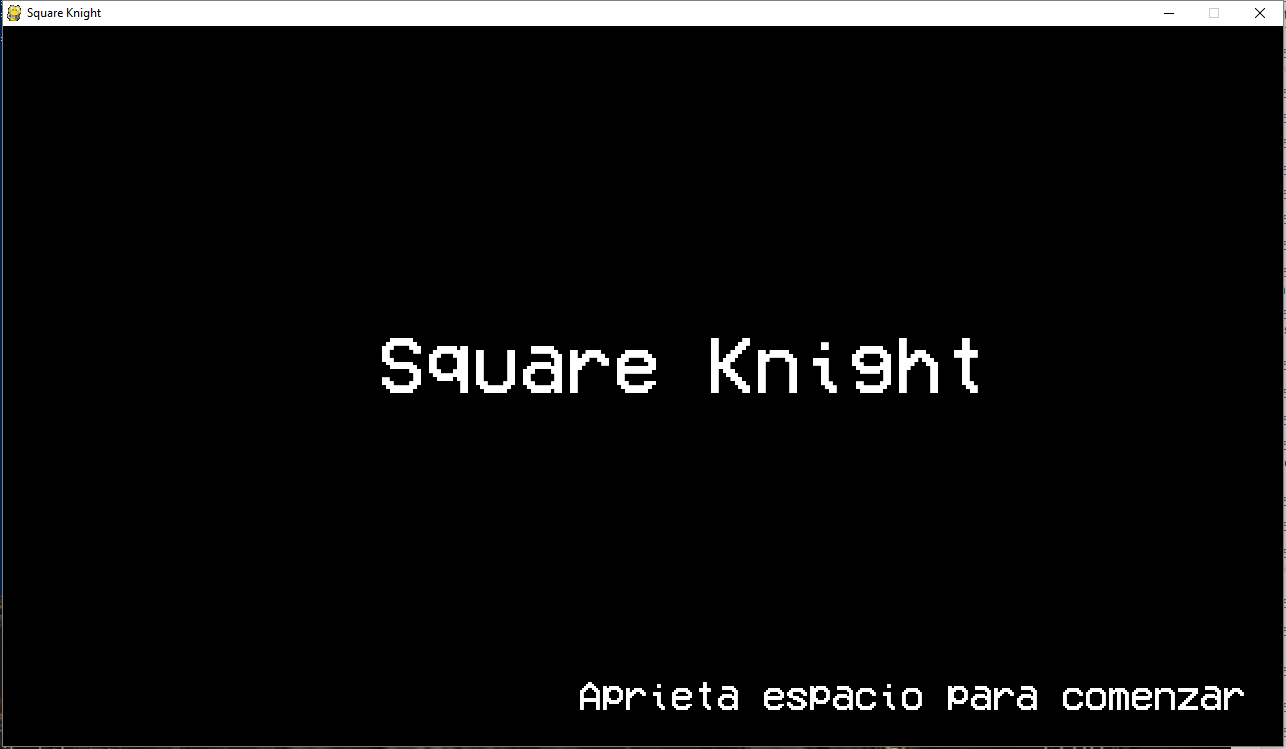
\includegraphics[width=0.30\textwidth]{images/screencap_01}
		\hfill
		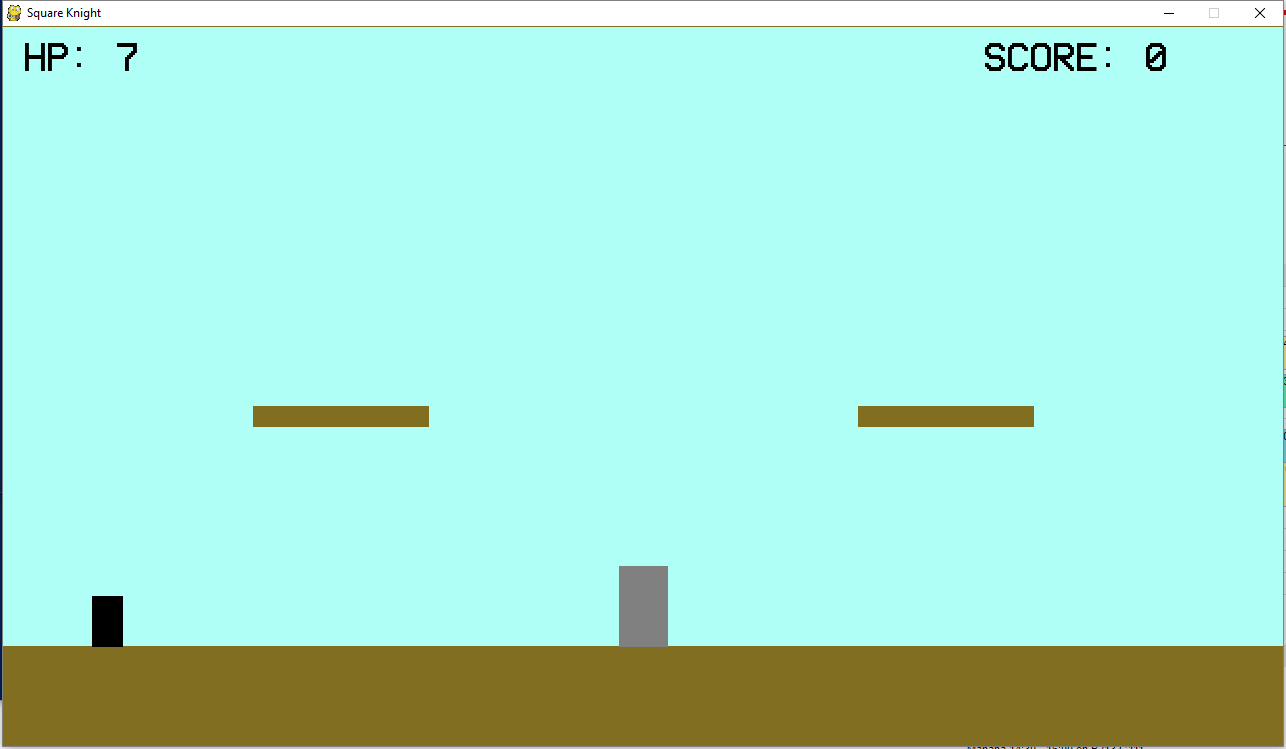
\includegraphics[width=0.30\textwidth]{images/screencap_02}
		\hfill
		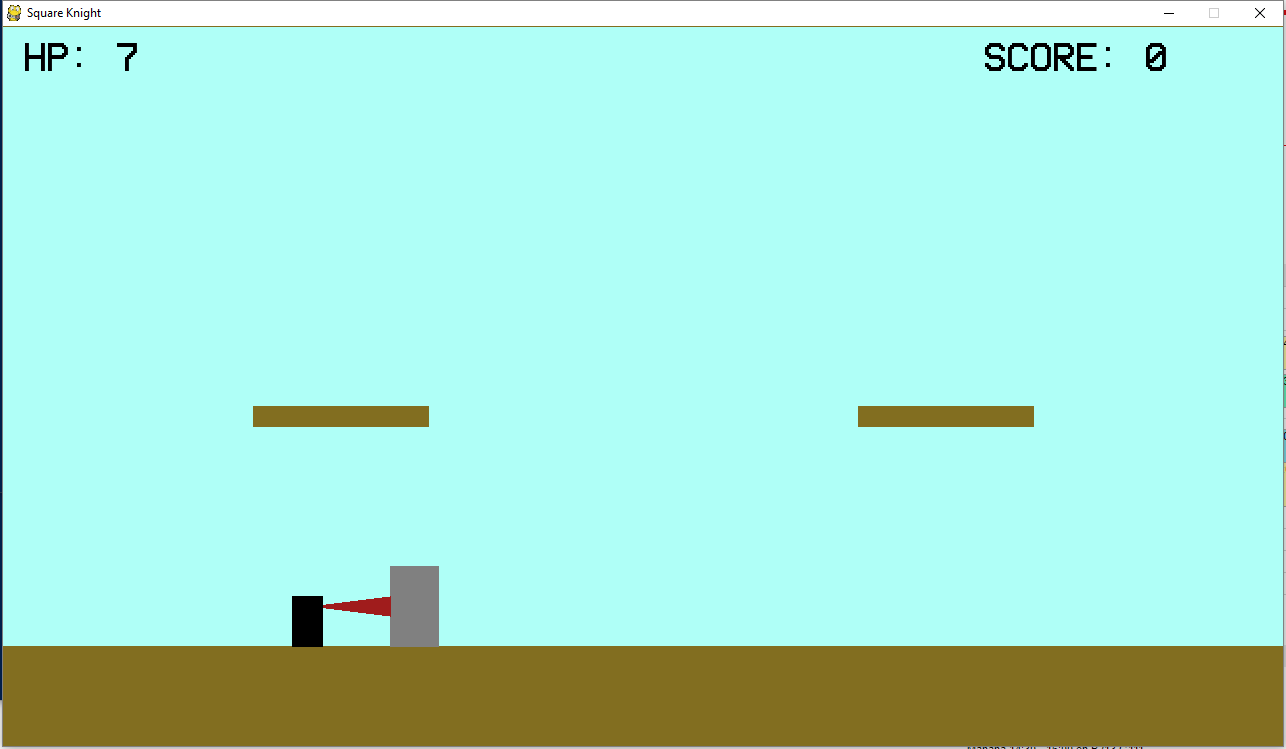
\includegraphics[width=0.30\textwidth]{images/screencap_03}
	\end{figure}

	\begin{figure}[H]
		\centering
		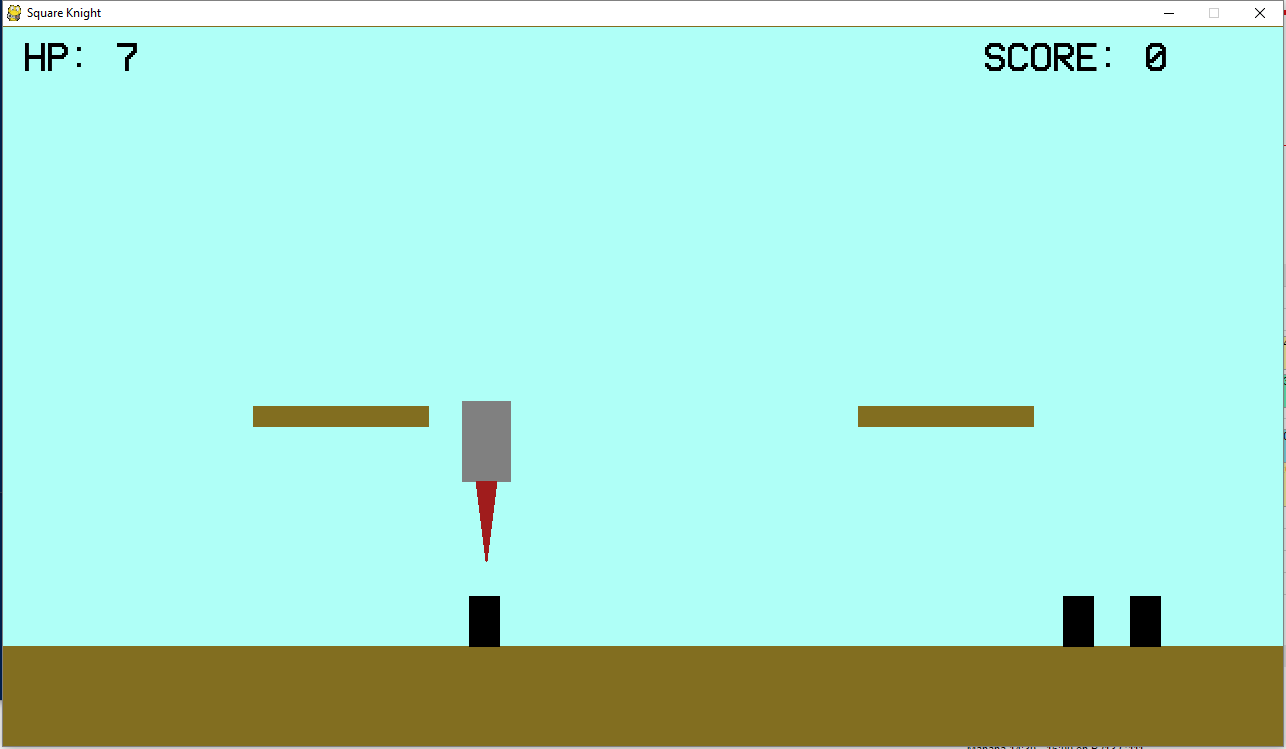
\includegraphics[width=0.30\textwidth]{images/screencap_04}
		\hfill
		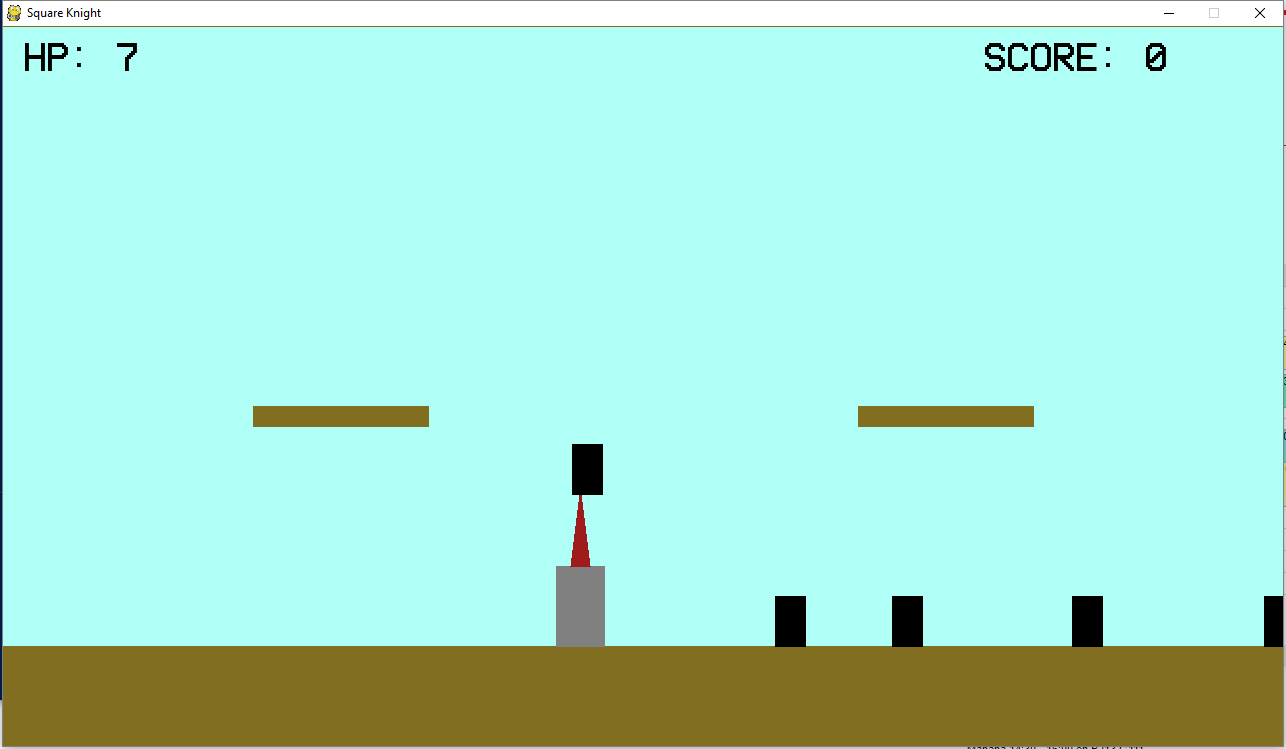
\includegraphics[width=0.30\textwidth]{images/screencap_05}
		\hfill
		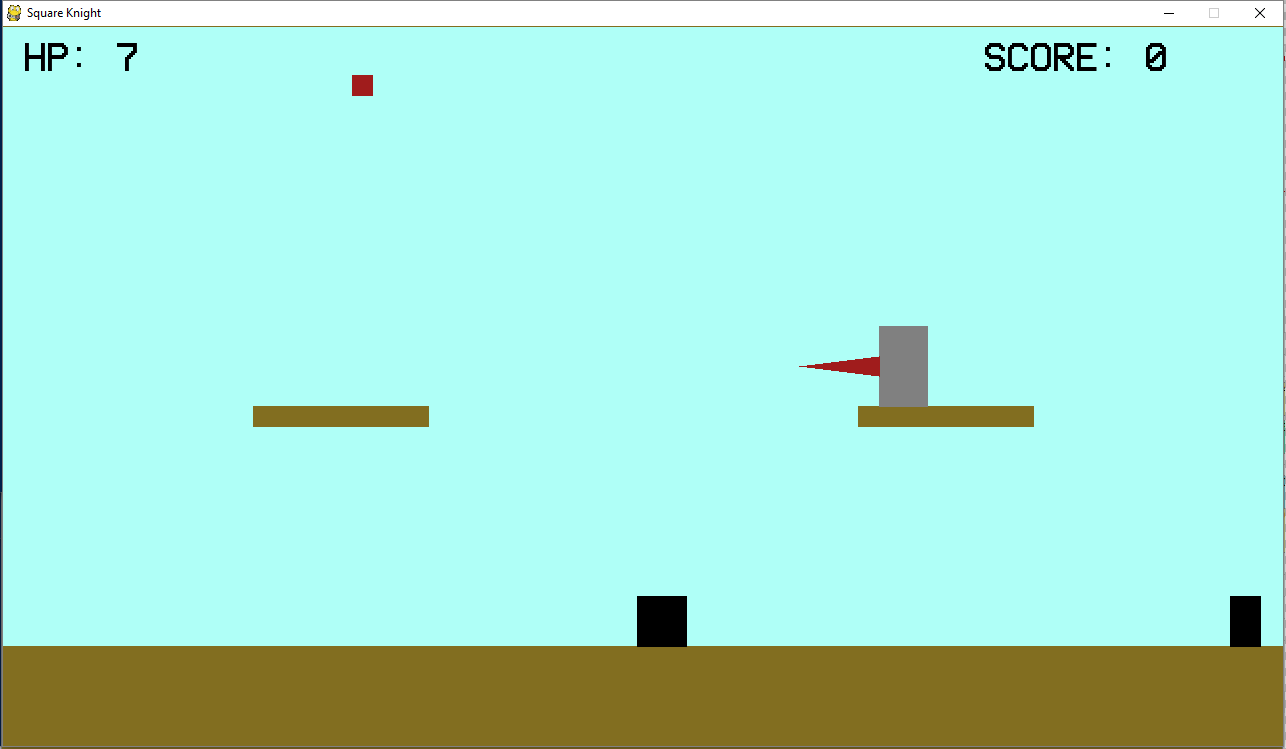
\includegraphics[width=0.30\textwidth]{images/screencap_06}
	\end{figure}

	\begin{figure}[H]
		\centering
		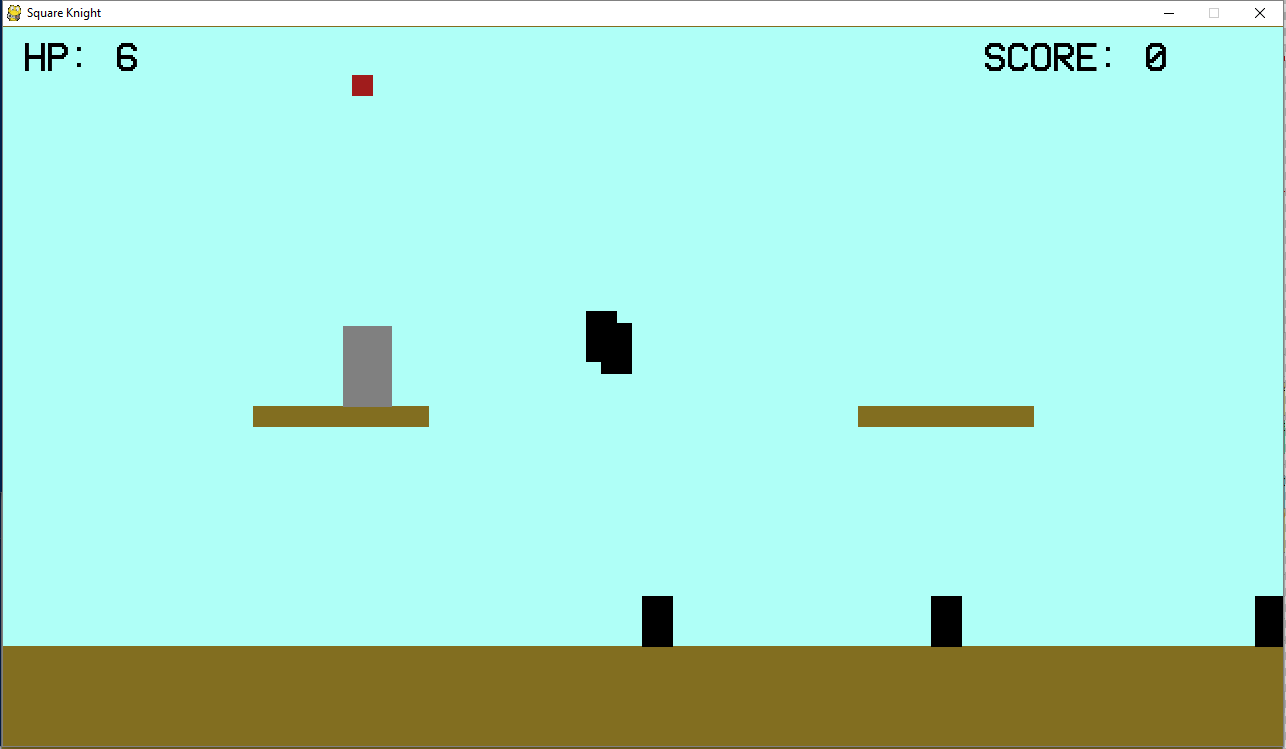
\includegraphics[width=0.30\textwidth]{images/screencap_07}
		\hfill
		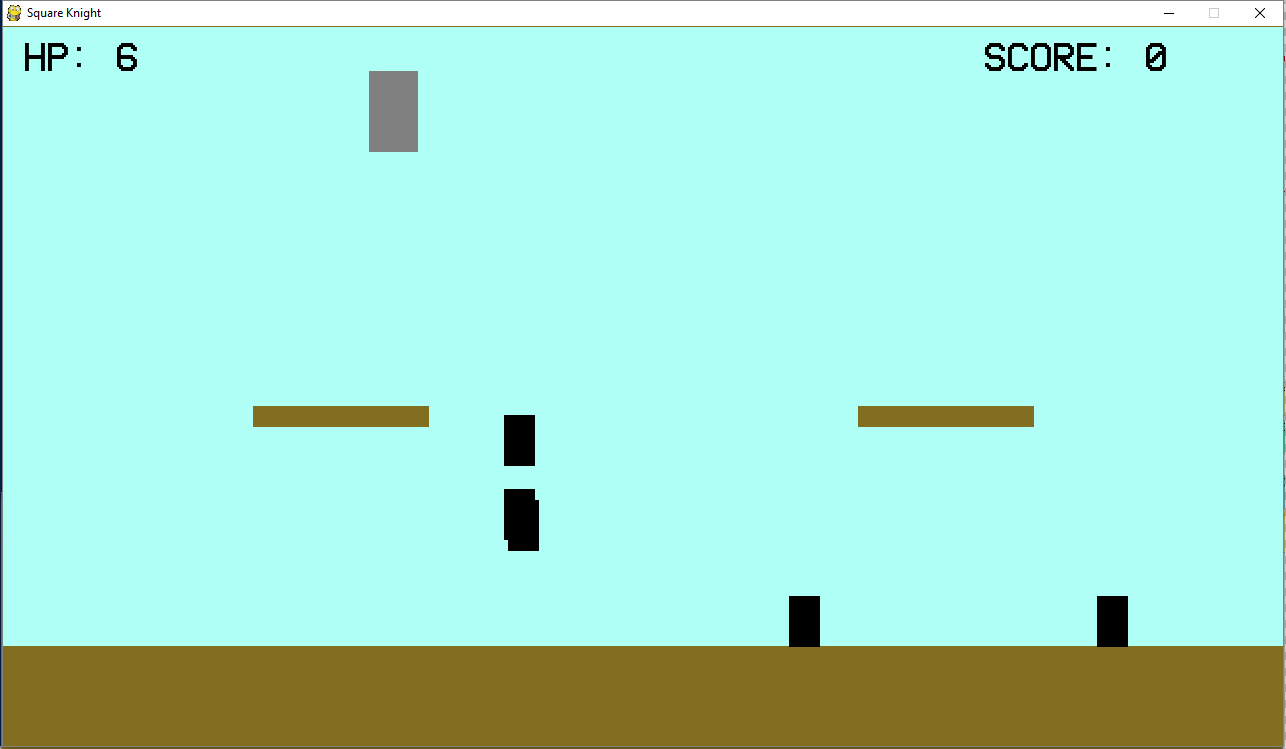
\includegraphics[width=0.30\textwidth]{images/screencap_08}
		\hfill
		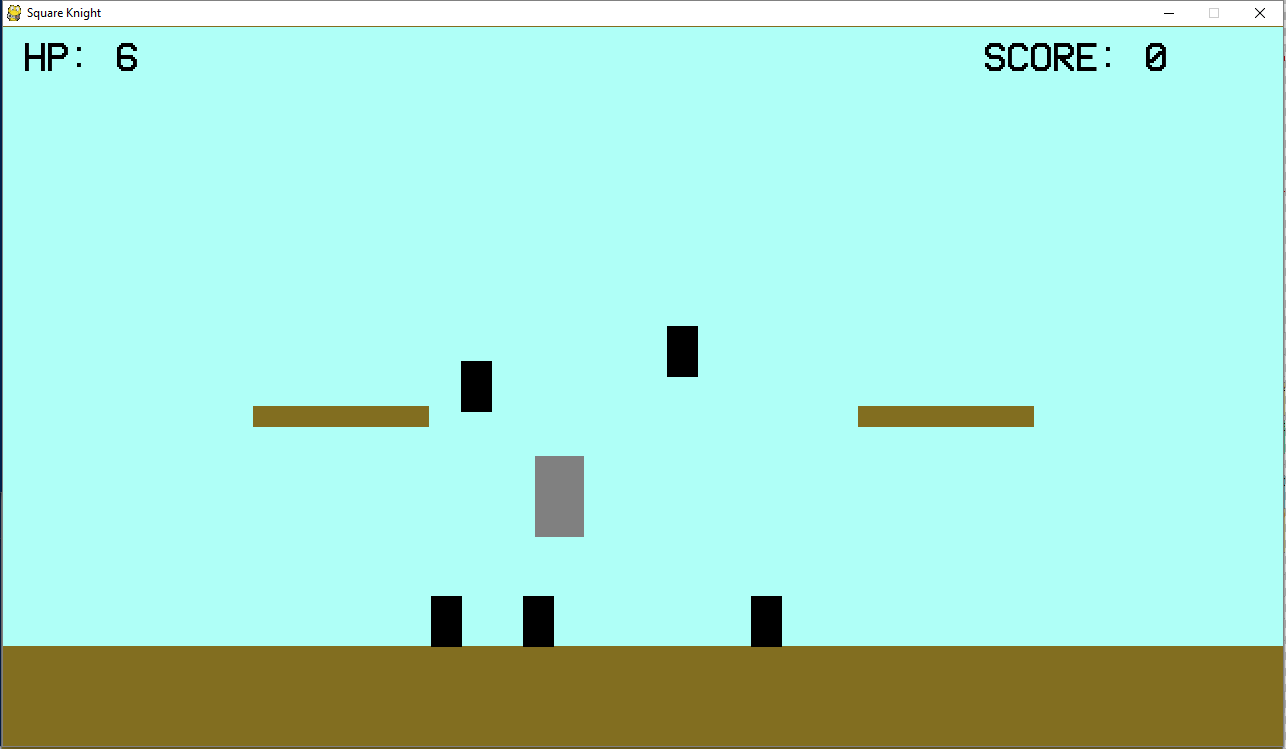
\includegraphics[width=0.30\textwidth]{images/screencap_09}
	\end{figure}

	\begin{figure}[H]
		\centering
		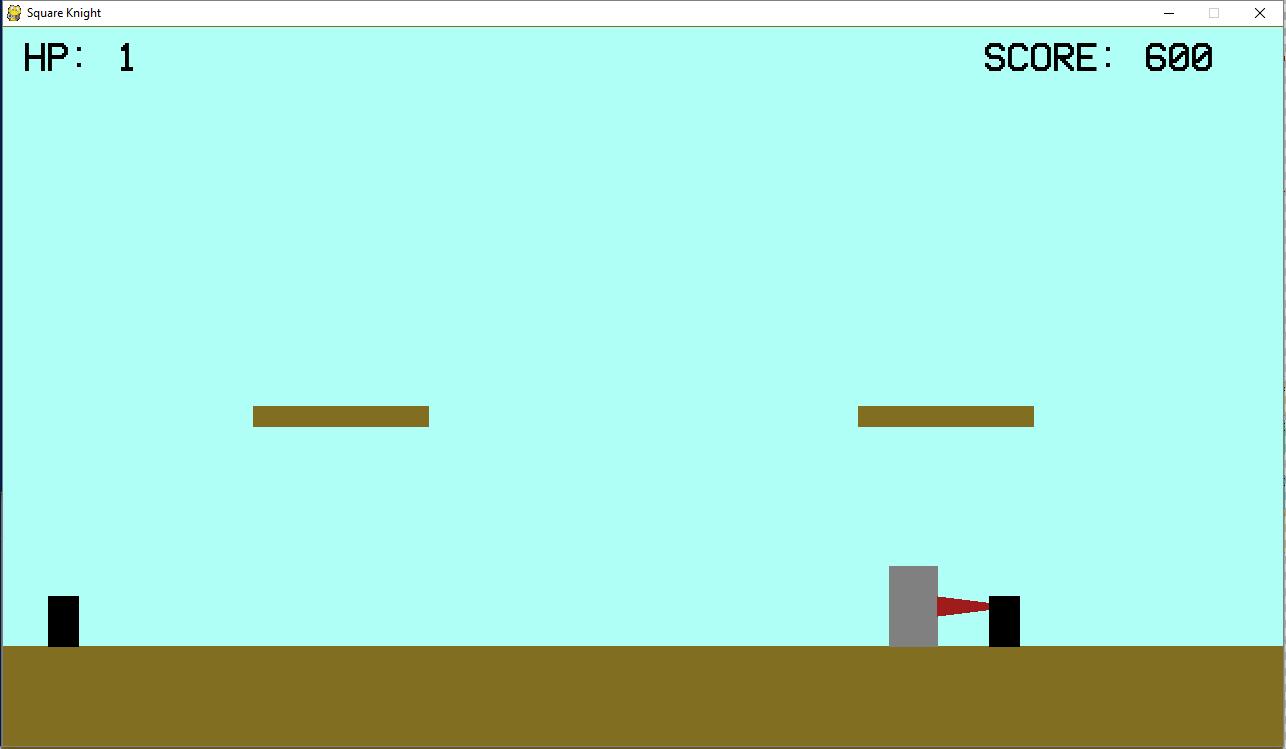
\includegraphics[width=0.30\textwidth]{images/screencap_10}
		\hfill
		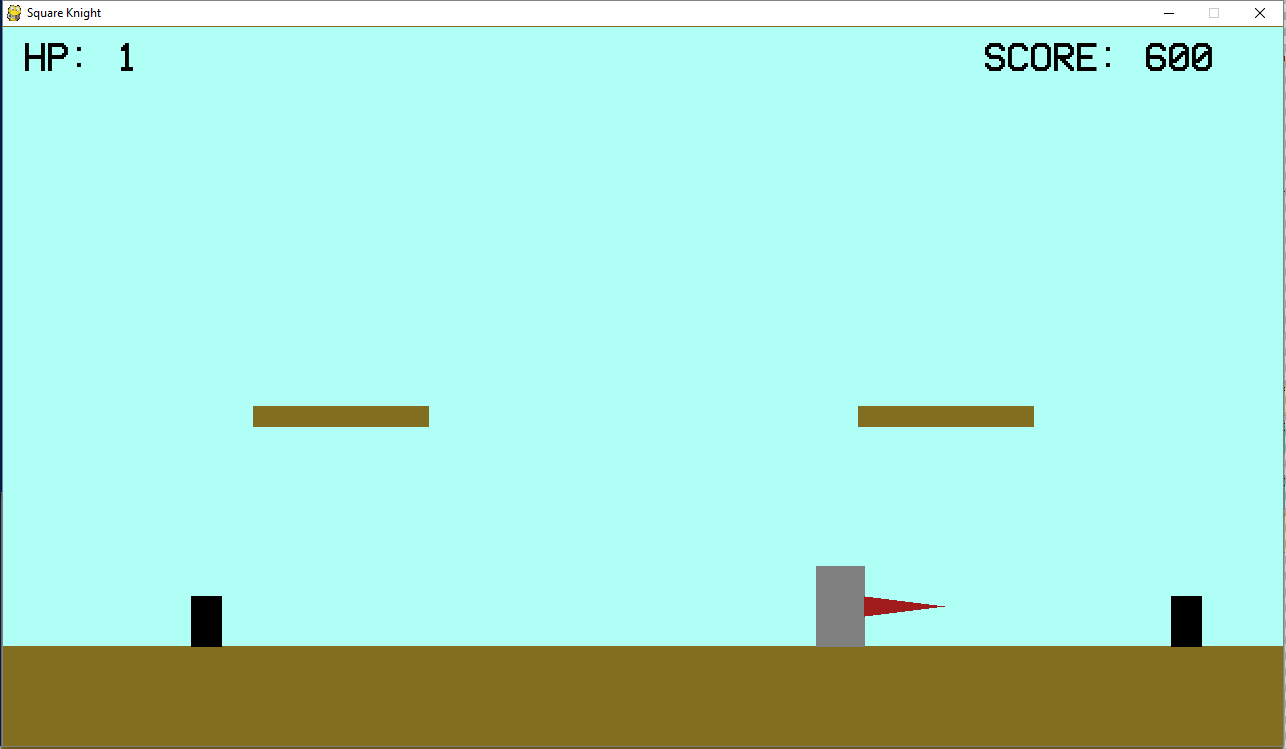
\includegraphics[width=0.30\textwidth]{images/screencap_11}
		\hfill
		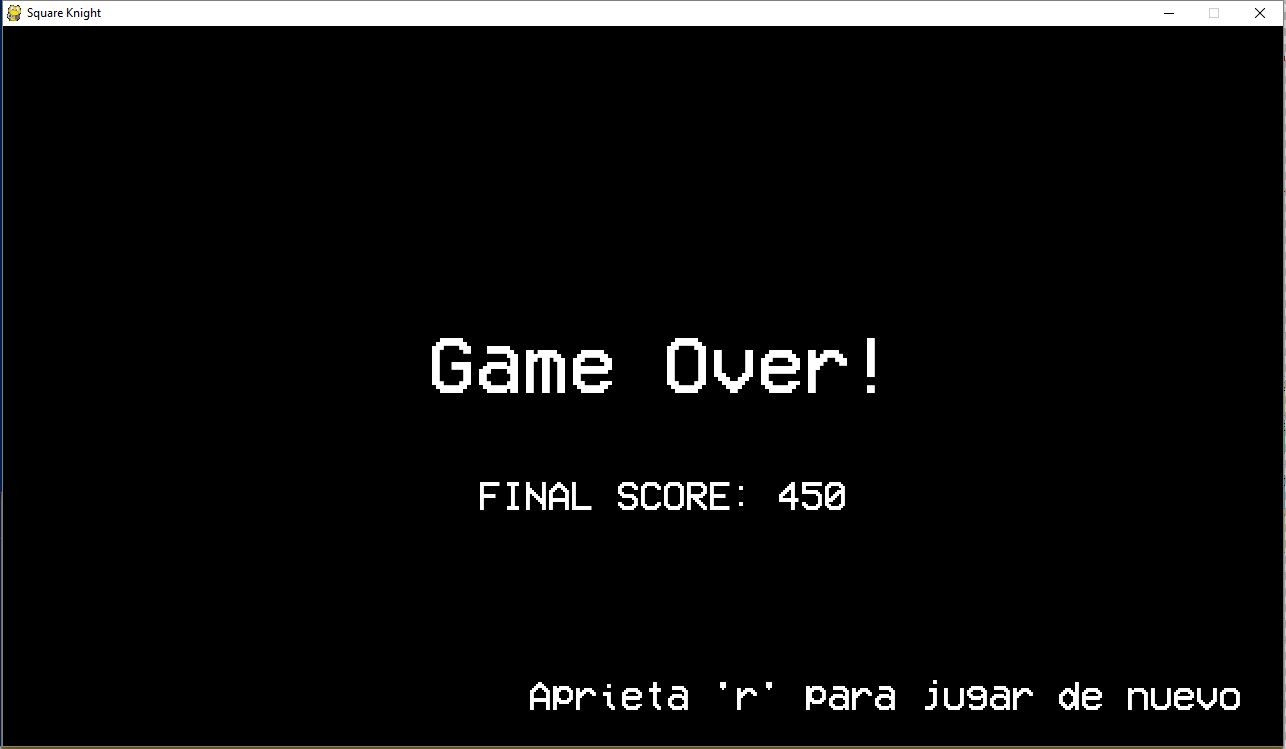
\includegraphics[width=0.30\textwidth]{images/screencap_12}
		\caption{Capturas del juego en acción.}
	\end{figure}

	Para probar el juego, por favor leer \verb!README.md!.

% FIN DEL DOCUMENTO
\end{document}